\section{Features \& Properties}
\label{sec:features}
This section reviews several important and useful properties of CC.
%and mostly new possibilities to CNN architecture design introduced by CC.
We show that introducing CC-layers gives rise to new CNN capabilities, and furthermore -- allows for \emph{new dynamic architectural designs determined at inference time}.

\textbf{A standard Conv-layer is a special case of the CC-Layer:}
Note that when the scale-factor $s=\nicefrac{1}{k}$, $k \in \mathbb{N}$, and $k$ has the same parity as the kernel support size in both dimensions, $g_n$ in Eq.~\ref{eq:grid} reduces to simple grid locations with integer pixel spacing between them. Thus, all output grid points share the same set of local distances to their discrete input ``Neighbors''. Hence, the set of weights are shared by all output `pixels', which is the case in standard convolution. This implies that  for integer scale ratios CC reduces to standard convolution, i.e.,  CC is a \emph{generalization} of the standard Conv-layer.

% \textbf{Collapsing back to standard convolution:} First we note that the distance of a grid point to the closest pixel center in the input determines the distances to all neighbors. This means that grid locations with same distance to closest `pixel' center share the same distances to neighbors and consequently will be mapped to the same set of weights. Considering this, we note that eq.~\ref{eq:grid} suggests that there are special cases. A scale-factor that is inverse of integer in both dimensions, produces grid locations with full `pixels' spacing between them, thus they all share the same distance to closest `pixel' center. As explained, the set of weights for each output `pixel' in such situations is identical. This implies that CC for such scale is actually a standard convolution, and shows that CC is a generalization of standard conv-layer.

\textbf{Dynamic scale-factor at inference:} As mentioned, the projected-grid is purely a function of the scale-factors and output shape. It is also important to note that in case of training the CC-layer with a \emph{random float scale factor}, we obtain a huge diversity of distances in $\varbold{\mathcal{D}}$ (see more details in Sec.~\ref{sec:train}). Hence the ``Internal-Net'' $\varbold{\mathcal{K}_\theta}$ which gets all the sub-`pixel' distances $\varbold{\mathcal{D}}$ as an input, and outputs a single kernel  consistent with them all,  must learn a  \emph{true continuous} weight function (the continuous kernel), independently of the scale factor or shape of the \ben{output}. Once it has recovered the continuous kernel (continuous weights),  CC can be applied at inference time to output any dynamically chosen scale or shape, simply by changing the sampling grid.

% \textbf{Cross-scale generalization:} Since the learning model $\mathcal{K}_\theta$ is unaware of the scale, it can be trained to one scale and generalize to another, under reasonable conditions. the scale trained on, cannot be a special case that collapses back to convolution, or a rational number with a denominator that is too small. In other words, generalization occurs over the distribution of distances between the grid and `pixel' centers. If this distribution collapses to a small set of possibilities then such generalization is damaged. A randomly selected float scale-factor will be able to generalize with probability ~1. 

\textbf{True Shift-Invariance/equivariance:} It was shown~\cite{zhang2019shiftinvar, azulay2018deep} that strided conv-layers \niv{lack}
% have damaged 
equivariance to shifts of the \ben{input}. This mostly happens due to aliasing. The common filter size tends to be smaller than the low-pass filter size required to remove high-frequencies when downscaling by a factor of 2. CC allows more gradual downscaling, so that (with the same kernel support) the sampling frequency is higher and less aliasing occurs. For example, one can replace a single strided convolution layer with downscaling-factor $s=1/2$, with a few (2-3) CC-layers, each with scale $1/2 < s < 1$ (e.g., 2 CC-layers with $s=1/\sqrt{{2}}$, or 3 CC-layers with $s=1/\sqrt[3]{{2}}$).

\textbf{Standard conv-layers often suffer from inherent misalignments, which are ameliorated by CC-layers:} Examining the accurate grid mapping in Eq.~\ref{eq:grid}, one can see that there are cases in standard discrete convolutions which fail to satisfy it. Such cases occur when the size of the filter and the stride have different parities, in some dimension. The intuitive reason is that the filter \emph{center} is defined by its parity: In odd-sized filters, the center of the output `pixel' falls on an input `pixel'-center, whereas in even-sized filter, it falls on the boundary between two input `pixels'. As mentioned, for a scale factor $1/int$, the set of weights is identical for any output position. Eq.~\ref{eq:grid} suggests that in such cases the grid locations are either all exactly on input `pixel' centers, or all on the boundary between input `pixels' (e.g., scale-factor of $\frac{1}{2}$ produces locations 0.5, 2.5, 4.5 etc., whereas scale factor of $\frac{1}{3}$ produces locations 1,4,7 etc.) This means that in case of an even scale with odd-sized filter, standard conv-layers introduce small misalignments between the input and output ($I$,$I'$). These small \benc{del: layer-to-layer} misalignments can accumulate to large misalignments over many layers. 

Such an example is shown in Fig.~\ref{fig:fig_missalign}. 
% Applying a fixed kernel for which the center of mass is the filter center, with a parity different than the scale will shift the result by half a `pixel'. Fig.~\ref{fig:fig_missalign} shows a simple experiment. 
We used a simple gaussian kernel,  and applied it repeatedly to an input image (white cross), using either a sequence of standard conv-layers or a sequence of CC-layers, all with stride=1 or scale=1, respectively. We chose an even-sized 4$\times$4 kernel. It can be seen that standard conv-layer shifts the result by half a pixel per iteration, resulting in a large shift after many iterations. In contrast, CC-based convolutions remain centered, due to the accurate sub-pixel grid mapping of Eq.~\ref{eq:grid}. Choosing a different padding method for the standard conv would only result in shifts to other directions; there is no way to apply a 4$\times$4 discrete convolution that keeps the same input size and does not induce misalignments. The reason neural networks still get good results is simple: they learn a variety of shifted kernels. This misalignment phenomenon has been observed in super-resolution works~\cite{zhang2020deep, ZSSR}. Still, the way  misalignments are currently addressed is non-ideal and unprincipled, as some portion of the filter size is not used and may create artifacts.

\textbf{Scale Ensembles:} Here we present \niv{an entirely}
% a totally 
new capability in Deep-Learning -- Dynamic Architectural Design of CNNs, at inference time, which is made possible by introducing multiple CC-layers into CNNs.  As mentioned before, a trained CC-layer can generate any output scale-factor chosen at inference time. Therefore, a single trained CNN which consists of multiple CC-layers, can be applied many times at inference, each time with \emph{a different sequence of scales}, as long as the final output scale \& shape of the entire network remain fixed. This means that there are infinitely many ways to apply such a trained network, and still get the same final output size/scale.  Moreover, each dimension (vertical or horizontal) can be scaled differently at intermediate CC-layers. This gives rise to a new type of ``self-ensembles'' of CNNs. We call it ``Scale Ensembles''.  Fig.~\ref{fig:scale_ensemble} schematically illustrates a few different scales-sequences for 3 consecutive CC-layers in the same pre-trained CNN. For example, the Green sequence applies 3 consecutive uniform scaling in both dimensions, same scaling each time; 
%, and uses a larger scale as the last one. 
the Blue sequence scales  the horizontal and vertical dimensions alternatingly; whereas the Red sequence offers yet another non-uniform sequence of scaling. At inference time we can apply the same pre-trained network several times, each with a different sequence of scales. We can then aggregate all the results of this ensemble,  to get an improved result  which is consistent with the entire ensemble. Aggregation can be achieved, e.g., by  averaging the class \niv{logits}
% probabilities 
in a classification task,  or by computing the median image of the ensemble in an image-processing task.

\begin{figure}
%\vspace*{-0.5cm}
\hspace{-0cm}
\centering
\begin{minipage}{.45\textwidth}
    \hspace{-1cm}
    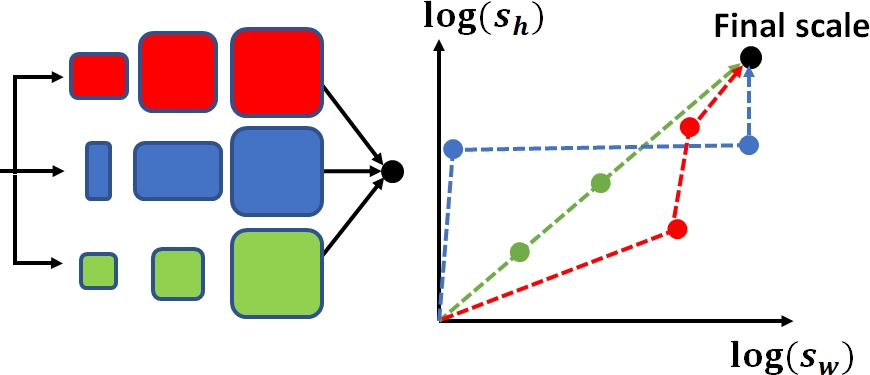
\includegraphics[width=1\textwidth]{figs/fig_scale_ensemble_Michal.jpg}
    \captionsetup{oneside, margin={-2cm,0cm}}
     \caption{\it ``Scale-Ensemble'' (see Sec.~\ref{sec:features}  for details).}
    \label{fig:scale_ensemble}
\end{minipage}%
  \hspace{0.3cm}
  \begin{minipage}{.3\textwidth}
  \centering
  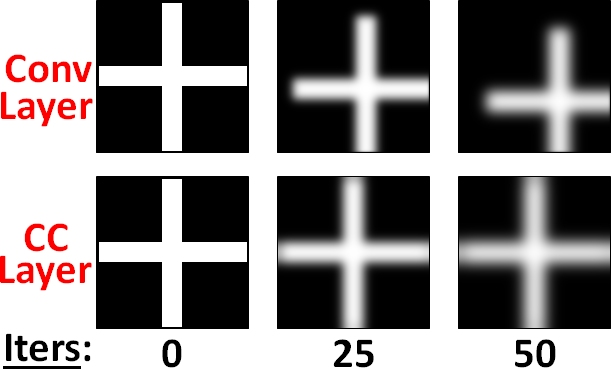
\includegraphics[width=1\textwidth]{figs/fig_misalign_Michal.jpg}
   \captionsetup{oneside, margin={-0.5cm,-1cm}}
  \caption{\it Standard conv-layers induce misalignments.  CC-layers do not.}
  \label{fig:fig_missalign}
    \end{minipage}
   \vspace*{-0.5cm}
\end{figure}